\subsection*{Equation d'onde}
\begin{equation*}
    u_{tt}=c^2u_{xx}
\end{equation*}
\textbf{Solution générale:}
\begin{equation*}
    \boxed{u(x,t)=f(x+ct)+g(x-ct)}
\end{equation*}
$f$ et $g$ sont deux fonction quelconques d'une seule variable.\\
\textbf{Solution avec condition initiales:}
\begin{equation*}
    \boxed{u(x,t)=\frac{1}{2}[\phi(x+ct)+\psi(x-ct)]+\frac{1}{2c}\int_{x-ct}^{x+ct}\psi(s)\mathrm{d}s}
\end{equation*}
\begin{figure}[H]
    \centering
    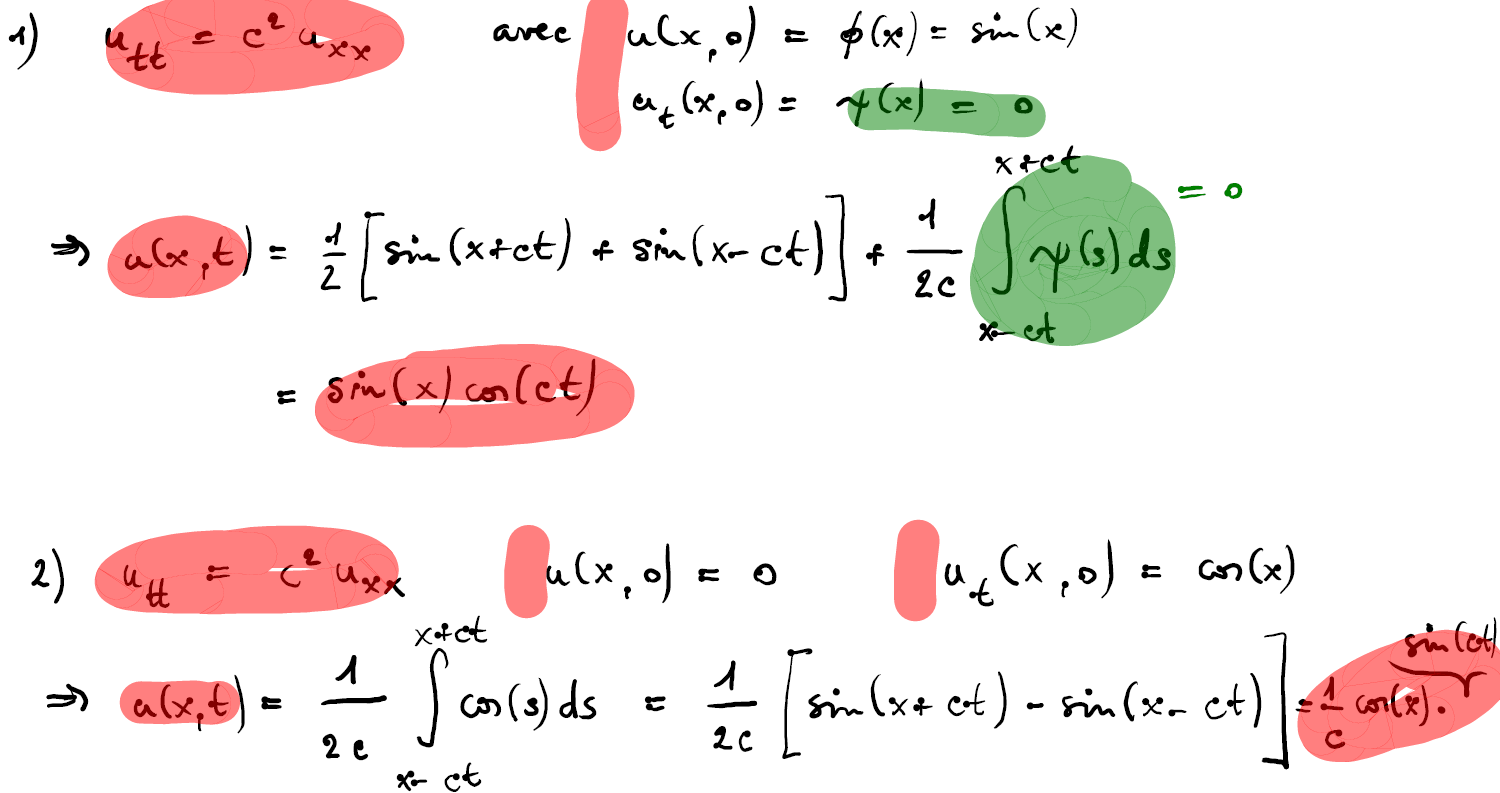
\includegraphics[width=\linewidth]{images/semaine2_onde.png}
\end{figure}